\documentclass[12pt, twoside]{article}
\usepackage[francais]{babel}
\usepackage[T1]{fontenc}
\usepackage[latin1]{inputenc}
\usepackage[left=7mm, right=7mm, top=3mm, bottom=3mm]{geometry}
\usepackage{float}
\usepackage{graphicx}
\usepackage{array}
\usepackage{multirow}
\usepackage{amsmath,amssymb,mathrsfs}
\usepackage{textcomp}
\pagestyle{empty}
\usepackage{soul}


\begin{document} 

NOM PRENOM: \ldots\ldots\ldots\ldots\ldots


\bigskip

\begin{center}
{\fbox{$4^{e}3$ \qquad \qquad \textbf{\Large{Mini-test 8 (sujet 1) }}
\qquad \qquad 17/04/2014}}
\end{center}

\textbf{Tous vos calculs doivent �tre �crits.}

\enskip

\ul{Exercice 1:} \textit{4 points}


\begin{tabular}{cc}
\begin{minipage}{11cm}
Le diagramme suivant donnne la r�partition des �l�ves d'un coll�ge selon leur
�ge.

\begin{enumerate}
  \item Faire un tableau d'effectif.
  \item Calculer l'�ge moyen d'un �l�ve de ce coll�ge.
  \item Quel est le pourcentage d'�l�ves ayant 15 ans ou plus?
\end{enumerate}
\end{minipage}
&
\begin{minipage}{7cm}
\begin{center}
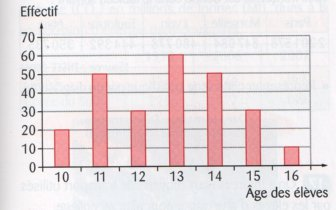
\includegraphics[width= 7cm]{images/age.jpg}
\end{center}
\end{minipage}
\end{tabular}


\bigskip

\ldots \ldots \ldots \ldots \ldots \ldots \ldots \ldots \ldots \ldots \ldots
\ldots \ldots \ldots \ldots \ldots \ldots \ldots \ldots \ldots \ldots \ldots
\ldots \ldots \ldots \ldots \ldots \ldots \ldots \ldots \ldots \ldots \ldots
\ldots \ldots 

\ldots \ldots \ldots \ldots \ldots \ldots \ldots \ldots \ldots \ldots \ldots
\ldots \ldots \ldots \ldots \ldots \ldots \ldots \ldots \ldots \ldots \ldots
\ldots \ldots \ldots \ldots \ldots \ldots \ldots \ldots \ldots \ldots \ldots
\ldots \ldots 

\ldots \ldots \ldots \ldots \ldots \ldots \ldots \ldots \ldots \ldots \ldots
\ldots \ldots \ldots \ldots \ldots \ldots \ldots \ldots \ldots \ldots \ldots
\ldots \ldots \ldots \ldots \ldots \ldots \ldots \ldots \ldots \ldots \ldots
\ldots \ldots 

\ldots \ldots \ldots \ldots \ldots \ldots \ldots \ldots \ldots \ldots \ldots
\ldots \ldots \ldots \ldots \ldots \ldots \ldots \ldots \ldots \ldots \ldots
\ldots \ldots \ldots \ldots \ldots \ldots \ldots \ldots \ldots \ldots \ldots
\ldots \ldots 

\ldots \ldots \ldots \ldots \ldots \ldots \ldots \ldots \ldots \ldots \ldots
\ldots \ldots \ldots \ldots \ldots \ldots \ldots \ldots \ldots \ldots \ldots
\ldots \ldots \ldots \ldots \ldots \ldots \ldots \ldots \ldots \ldots \ldots
\ldots \ldots 

\ldots \ldots \ldots \ldots \ldots \ldots \ldots \ldots \ldots \ldots \ldots
\ldots \ldots \ldots \ldots \ldots \ldots \ldots \ldots \ldots \ldots \ldots
\ldots \ldots \ldots \ldots \ldots \ldots \ldots \ldots \ldots \ldots \ldots
\ldots \ldots 

\ldots \ldots \ldots \ldots \ldots \ldots \ldots \ldots \ldots \ldots \ldots
\ldots \ldots \ldots \ldots \ldots \ldots \ldots \ldots \ldots \ldots \ldots
\ldots \ldots \ldots \ldots \ldots \ldots \ldots \ldots \ldots \ldots \ldots
\ldots \ldots 

\ldots \ldots \ldots \ldots \ldots \ldots \ldots \ldots \ldots \ldots \ldots
\ldots \ldots \ldots \ldots \ldots \ldots \ldots \ldots \ldots \ldots \ldots
\ldots \ldots \ldots \ldots \ldots \ldots \ldots \ldots \ldots \ldots \ldots
\ldots \ldots 

\ldots \ldots \ldots \ldots \ldots \ldots \ldots \ldots \ldots \ldots \ldots
\ldots \ldots \ldots \ldots \ldots \ldots \ldots \ldots \ldots \ldots \ldots
\ldots \ldots \ldots \ldots \ldots \ldots \ldots \ldots \ldots \ldots \ldots
\ldots \ldots 



\bigskip




\ul{Exercice 2:} \textit{6 points}

\enskip

Dans un village o� la vitesse est limit�e � 50km/h, les gendarmes ont relev�
les vitesses suivantes:

\enskip

45 \quad 54 \quad 48 \quad 50 \quad 45 \quad 57 \quad  42 \quad 42 \quad  54
\quad 52 \quad 37 \quad 57 \quad 57 \quad 49 \quad 50 \quad 52 \quad 46 \quad
57 \quad  30 \quad 51 \quad 43 \quad 49 \quad 54 \quad 52 \quad 35 \quad 48
\quad 45 \quad 54 \quad 30 \quad 48 \quad 30 \quad 54


\begin{enumerate}
  \item Quel est l'effectif total?
  \item Faire un tableau d'effectifs.
  \item Calculer la moyenne des vitesses relev�es de deux mani�res diff�rentes.
  \item Quelle est la fr�quence (en \%) des v�hicules en infraction?
\end{enumerate}



\ldots \ldots \ldots \ldots \ldots \ldots \ldots \ldots \ldots \ldots \ldots
\ldots \ldots \ldots \ldots \ldots \ldots \ldots \ldots \ldots \ldots \ldots
\ldots \ldots \ldots \ldots \ldots \ldots \ldots \ldots \ldots \ldots \ldots
\ldots \ldots 

\ldots \ldots \ldots \ldots \ldots \ldots \ldots \ldots \ldots \ldots \ldots
\ldots \ldots \ldots \ldots \ldots \ldots \ldots \ldots \ldots \ldots \ldots
\ldots \ldots \ldots \ldots \ldots \ldots \ldots \ldots \ldots \ldots \ldots
\ldots \ldots 

\ldots \ldots \ldots \ldots \ldots \ldots \ldots \ldots \ldots \ldots \ldots
\ldots \ldots \ldots \ldots \ldots \ldots \ldots \ldots \ldots \ldots \ldots
\ldots \ldots \ldots \ldots \ldots \ldots \ldots \ldots \ldots \ldots \ldots
\ldots \ldots 

\ldots \ldots \ldots \ldots \ldots \ldots \ldots \ldots \ldots \ldots \ldots
\ldots \ldots \ldots \ldots \ldots \ldots \ldots \ldots \ldots \ldots \ldots
\ldots \ldots \ldots \ldots \ldots \ldots \ldots \ldots \ldots \ldots \ldots
\ldots \ldots 

\ldots \ldots \ldots \ldots \ldots \ldots \ldots \ldots \ldots \ldots \ldots
\ldots \ldots \ldots \ldots \ldots \ldots \ldots \ldots \ldots \ldots \ldots
\ldots \ldots \ldots \ldots \ldots \ldots \ldots \ldots \ldots \ldots \ldots
\ldots \ldots 

\ldots \ldots \ldots \ldots \ldots \ldots \ldots \ldots \ldots \ldots \ldots
\ldots \ldots \ldots \ldots \ldots \ldots \ldots \ldots \ldots \ldots \ldots
\ldots \ldots \ldots \ldots \ldots \ldots \ldots \ldots \ldots \ldots \ldots
\ldots \ldots 

\ldots \ldots \ldots \ldots \ldots \ldots \ldots \ldots \ldots \ldots \ldots
\ldots \ldots \ldots \ldots \ldots \ldots \ldots \ldots \ldots \ldots \ldots
\ldots \ldots \ldots \ldots \ldots \ldots \ldots \ldots \ldots \ldots \ldots
\ldots \ldots 

\ldots \ldots \ldots \ldots \ldots \ldots \ldots \ldots \ldots \ldots \ldots
\ldots \ldots \ldots \ldots \ldots \ldots \ldots \ldots \ldots \ldots \ldots
\ldots \ldots \ldots \ldots \ldots \ldots \ldots \ldots \ldots \ldots \ldots
\ldots \ldots 

\ldots \ldots \ldots \ldots \ldots \ldots \ldots \ldots \ldots \ldots \ldots
\ldots \ldots \ldots \ldots \ldots \ldots \ldots \ldots \ldots \ldots \ldots
\ldots \ldots \ldots \ldots \ldots \ldots \ldots \ldots \ldots \ldots \ldots
\ldots \ldots 

\ldots \ldots \ldots \ldots \ldots \ldots \ldots \ldots \ldots \ldots \ldots
\ldots \ldots \ldots \ldots \ldots \ldots \ldots \ldots \ldots \ldots \ldots
\ldots \ldots \ldots \ldots \ldots \ldots \ldots \ldots \ldots \ldots \ldots
\ldots \ldots 

\ldots \ldots \ldots \ldots \ldots \ldots \ldots \ldots \ldots \ldots \ldots
\ldots \ldots \ldots \ldots \ldots \ldots \ldots \ldots \ldots \ldots \ldots
\ldots \ldots \ldots \ldots \ldots \ldots \ldots \ldots \ldots \ldots \ldots
\ldots \ldots 

\ldots \ldots \ldots \ldots \ldots \ldots \ldots \ldots \ldots \ldots \ldots
\ldots \ldots \ldots \ldots \ldots \ldots \ldots \ldots \ldots \ldots \ldots
\ldots \ldots \ldots \ldots \ldots \ldots \ldots \ldots \ldots \ldots \ldots
\ldots \ldots 

\ldots \ldots \ldots \ldots \ldots \ldots \ldots \ldots \ldots \ldots \ldots
\ldots \ldots \ldots \ldots \ldots \ldots \ldots \ldots \ldots \ldots \ldots
\ldots \ldots \ldots \ldots \ldots \ldots \ldots \ldots \ldots \ldots \ldots
\ldots \ldots 

\ldots \ldots \ldots \ldots \ldots \ldots \ldots \ldots \ldots \ldots \ldots
\ldots \ldots \ldots \ldots \ldots \ldots \ldots \ldots \ldots \ldots \ldots
\ldots \ldots \ldots \ldots \ldots \ldots \ldots \ldots \ldots \ldots \ldots
\ldots \ldots 

\ldots \ldots \ldots \ldots \ldots \ldots \ldots \ldots \ldots \ldots \ldots
\ldots \ldots \ldots \ldots \ldots \ldots \ldots \ldots \ldots \ldots \ldots
\ldots \ldots \ldots \ldots \ldots \ldots \ldots \ldots \ldots \ldots \ldots
\ldots \ldots 

\ldots \ldots \ldots \ldots \ldots \ldots \ldots \ldots \ldots \ldots \ldots
\ldots \ldots \ldots \ldots \ldots \ldots \ldots \ldots \ldots \ldots \ldots
\ldots \ldots \ldots \ldots \ldots \ldots \ldots \ldots \ldots \ldots \ldots
\ldots \ldots 

\pagebreak


NOM PRENOM: \ldots\ldots\ldots\ldots\ldots


\bigskip

\begin{center}
{\fbox{$4^{e}3$ \qquad \qquad \textbf{\Large{Mini-test 8 (sujet 2) }}
\qquad \qquad 17/04/2014}}
\end{center}

\textbf{Tous vos calculs doivent �tre �crits.}

\enskip

\ul{Exercice 1:} \textit{4 points}


\begin{tabular}{cc}
\begin{minipage}{11cm}
Le diagramme suivant donnne la r�partition des �l�ves d'un coll�ge selon leur
�ge.

\begin{enumerate}
  \item Faire un tableau d'effectif.
  \item Calculer l'�ge moyen d'un �l�ve de ce coll�ge.
  \item Quel est le pourcentage d'�l�ves ayant 11 ans ou moins?
\end{enumerate}
\end{minipage}
&
\begin{minipage}{7cm}
\begin{center}
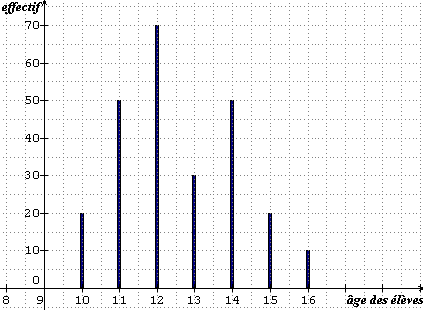
\includegraphics[width= 7cm]{images/ex12.png}
\end{center}
\end{minipage}
\end{tabular}


\bigskip


\ldots \ldots \ldots \ldots \ldots \ldots \ldots \ldots \ldots \ldots \ldots
\ldots \ldots \ldots \ldots \ldots \ldots \ldots \ldots \ldots \ldots \ldots
\ldots \ldots \ldots \ldots \ldots \ldots \ldots \ldots \ldots \ldots \ldots
\ldots \ldots 

\ldots \ldots \ldots \ldots \ldots \ldots \ldots \ldots \ldots \ldots \ldots
\ldots \ldots \ldots \ldots \ldots \ldots \ldots \ldots \ldots \ldots \ldots
\ldots \ldots \ldots \ldots \ldots \ldots \ldots \ldots \ldots \ldots \ldots
\ldots \ldots 

\ldots \ldots \ldots \ldots \ldots \ldots \ldots \ldots \ldots \ldots \ldots
\ldots \ldots \ldots \ldots \ldots \ldots \ldots \ldots \ldots \ldots \ldots
\ldots \ldots \ldots \ldots \ldots \ldots \ldots \ldots \ldots \ldots \ldots
\ldots \ldots 

\ldots \ldots \ldots \ldots \ldots \ldots \ldots \ldots \ldots \ldots \ldots
\ldots \ldots \ldots \ldots \ldots \ldots \ldots \ldots \ldots \ldots \ldots
\ldots \ldots \ldots \ldots \ldots \ldots \ldots \ldots \ldots \ldots \ldots
\ldots \ldots 

\ldots \ldots \ldots \ldots \ldots \ldots \ldots \ldots \ldots \ldots \ldots
\ldots \ldots \ldots \ldots \ldots \ldots \ldots \ldots \ldots \ldots \ldots
\ldots \ldots \ldots \ldots \ldots \ldots \ldots \ldots \ldots \ldots \ldots
\ldots \ldots 

\ldots \ldots \ldots \ldots \ldots \ldots \ldots \ldots \ldots \ldots \ldots
\ldots \ldots \ldots \ldots \ldots \ldots \ldots \ldots \ldots \ldots \ldots
\ldots \ldots \ldots \ldots \ldots \ldots \ldots \ldots \ldots \ldots \ldots
\ldots \ldots 

\ldots \ldots \ldots \ldots \ldots \ldots \ldots \ldots \ldots \ldots \ldots
\ldots \ldots \ldots \ldots \ldots \ldots \ldots \ldots \ldots \ldots \ldots
\ldots \ldots \ldots \ldots \ldots \ldots \ldots \ldots \ldots \ldots \ldots
\ldots \ldots 

\ldots \ldots \ldots \ldots \ldots \ldots \ldots \ldots \ldots \ldots \ldots
\ldots \ldots \ldots \ldots \ldots \ldots \ldots \ldots \ldots \ldots \ldots
\ldots \ldots \ldots \ldots \ldots \ldots \ldots \ldots \ldots \ldots \ldots
\ldots \ldots 



\bigskip




\ul{Exercice 2:} \textit{6 points}

\enskip

Dans un village o� la vitesse est limit�e � 50km/h, les gendarmes ont relev�
les vitesses suivantes:

\enskip

46 \quad 53 \quad 49 \quad 50 \quad 45 \quad 58 \quad  41 \quad 41 \quad  53
\quad 52 \quad 36 \quad 58 \quad 58 \quad 49 \quad 50 \quad 52 \quad 46 \quad
58 \quad  30 \quad 51 \quad 43 \quad 49 \quad 53 \quad 52 \quad 35 \quad 48
\quad 46 \quad 53 \quad 30 \quad 48 \quad 30 \quad 53 \quad 50 \quad 45


\begin{enumerate}
  \item Quel est l'effectif total?
  \item Faire un tableau d'effectifs.
  \item Calculer la moyenne des vitesses relev�es de deux mani�res diff�rentes.
  \item Quelle est la fr�quence (en \%) des v�hicules en infraction?
\end{enumerate}



\ldots \ldots \ldots \ldots \ldots \ldots \ldots \ldots \ldots \ldots \ldots
\ldots \ldots \ldots \ldots \ldots \ldots \ldots \ldots \ldots \ldots \ldots
\ldots \ldots \ldots \ldots \ldots \ldots \ldots \ldots \ldots \ldots \ldots
\ldots \ldots 

\ldots \ldots \ldots \ldots \ldots \ldots \ldots \ldots \ldots \ldots \ldots
\ldots \ldots \ldots \ldots \ldots \ldots \ldots \ldots \ldots \ldots \ldots
\ldots \ldots \ldots \ldots \ldots \ldots \ldots \ldots \ldots \ldots \ldots
\ldots \ldots 

\ldots \ldots \ldots \ldots \ldots \ldots \ldots \ldots \ldots \ldots \ldots
\ldots \ldots \ldots \ldots \ldots \ldots \ldots \ldots \ldots \ldots \ldots
\ldots \ldots \ldots \ldots \ldots \ldots \ldots \ldots \ldots \ldots \ldots
\ldots \ldots 

\ldots \ldots \ldots \ldots \ldots \ldots \ldots \ldots \ldots \ldots \ldots
\ldots \ldots \ldots \ldots \ldots \ldots \ldots \ldots \ldots \ldots \ldots
\ldots \ldots \ldots \ldots \ldots \ldots \ldots \ldots \ldots \ldots \ldots
\ldots \ldots 

\ldots \ldots \ldots \ldots \ldots \ldots \ldots \ldots \ldots \ldots \ldots
\ldots \ldots \ldots \ldots \ldots \ldots \ldots \ldots \ldots \ldots \ldots
\ldots \ldots \ldots \ldots \ldots \ldots \ldots \ldots \ldots \ldots \ldots
\ldots \ldots 

\ldots \ldots \ldots \ldots \ldots \ldots \ldots \ldots \ldots \ldots \ldots
\ldots \ldots \ldots \ldots \ldots \ldots \ldots \ldots \ldots \ldots \ldots
\ldots \ldots \ldots \ldots \ldots \ldots \ldots \ldots \ldots \ldots \ldots
\ldots \ldots 

\ldots \ldots \ldots \ldots \ldots \ldots \ldots \ldots \ldots \ldots \ldots
\ldots \ldots \ldots \ldots \ldots \ldots \ldots \ldots \ldots \ldots \ldots
\ldots \ldots \ldots \ldots \ldots \ldots \ldots \ldots \ldots \ldots \ldots
\ldots \ldots 

\ldots \ldots \ldots \ldots \ldots \ldots \ldots \ldots \ldots \ldots \ldots
\ldots \ldots \ldots \ldots \ldots \ldots \ldots \ldots \ldots \ldots \ldots
\ldots \ldots \ldots \ldots \ldots \ldots \ldots \ldots \ldots \ldots \ldots
\ldots \ldots 

\ldots \ldots \ldots \ldots \ldots \ldots \ldots \ldots \ldots \ldots \ldots
\ldots \ldots \ldots \ldots \ldots \ldots \ldots \ldots \ldots \ldots \ldots
\ldots \ldots \ldots \ldots \ldots \ldots \ldots \ldots \ldots \ldots \ldots
\ldots \ldots 

\ldots \ldots \ldots \ldots \ldots \ldots \ldots \ldots \ldots \ldots \ldots
\ldots \ldots \ldots \ldots \ldots \ldots \ldots \ldots \ldots \ldots \ldots
\ldots \ldots \ldots \ldots \ldots \ldots \ldots \ldots \ldots \ldots \ldots
\ldots \ldots 

\ldots \ldots \ldots \ldots \ldots \ldots \ldots \ldots \ldots \ldots \ldots
\ldots \ldots \ldots \ldots \ldots \ldots \ldots \ldots \ldots \ldots \ldots
\ldots \ldots \ldots \ldots \ldots \ldots \ldots \ldots \ldots \ldots \ldots
\ldots \ldots 

\ldots \ldots \ldots \ldots \ldots \ldots \ldots \ldots \ldots \ldots \ldots
\ldots \ldots \ldots \ldots \ldots \ldots \ldots \ldots \ldots \ldots \ldots
\ldots \ldots \ldots \ldots \ldots \ldots \ldots \ldots \ldots \ldots \ldots
\ldots \ldots 

\ldots \ldots \ldots \ldots \ldots \ldots \ldots \ldots \ldots \ldots \ldots
\ldots \ldots \ldots \ldots \ldots \ldots \ldots \ldots \ldots \ldots \ldots
\ldots \ldots \ldots \ldots \ldots \ldots \ldots \ldots \ldots \ldots \ldots
\ldots \ldots 

\ldots \ldots \ldots \ldots \ldots \ldots \ldots \ldots \ldots \ldots \ldots
\ldots \ldots \ldots \ldots \ldots \ldots \ldots \ldots \ldots \ldots \ldots
\ldots \ldots \ldots \ldots \ldots \ldots \ldots \ldots \ldots \ldots \ldots
\ldots \ldots 

\ldots \ldots \ldots \ldots \ldots \ldots \ldots \ldots \ldots \ldots \ldots
\ldots \ldots \ldots \ldots \ldots \ldots \ldots \ldots \ldots \ldots \ldots
\ldots \ldots \ldots \ldots \ldots \ldots \ldots \ldots \ldots \ldots \ldots
\ldots \ldots 

\ldots \ldots \ldots \ldots \ldots \ldots \ldots \ldots \ldots \ldots \ldots
\ldots \ldots \ldots \ldots \ldots \ldots \ldots \ldots \ldots \ldots \ldots
\ldots \ldots \ldots \ldots \ldots \ldots \ldots \ldots \ldots \ldots \ldots
\ldots \ldots
\end{document}
